\section{Data Organization and Problem Formulation}\label{sec:problem formulation}

This section describes the hybrid organization of high-order element data and formulates the data-reduction problem considered in this work.

\subsection{Organization of High-Order Element Data}\label{sec:problem formulation:data characteristics}

Although simulation systems such as NekRS~\cite{fischer2022nekrs}, MFEM~\cite{anderson2021mfem}, and Nektar++~\cite{moxey2020nektar++} use different file formats, their output fields share an organization determined by the underlying element discretization. We use the following common logical representation for one scalar field:
\begin{equation}
X=\{x_{e,i,j,k}\}\in\mathbb{R}^{E\times n_x\times n_y\times n_z},
\label{eq:logical-representation}
\end{equation}
where $E$ is the number of elements, $e$ is the element index, and $(i,j,k)$ identifies a local position within an element. The element index follows the stored order rather than a fixed multidimensional layout, so consecutive values of $e$ do not necessarily identify physically adjacent elements.

In a three-dimensional simulation, the elements are commonly geometrically deformed hexahedra connected through shared faces. In a two-dimensional simulation, they are deformed quadrilaterals connected through shared edges. Globally, this connectivity is unstructured. Figure~\ref{fig:characterizing-hohs}(a) illustrates three connected hexahedral elements in such a mesh.

\begin{figure}[htb]
    \centering
    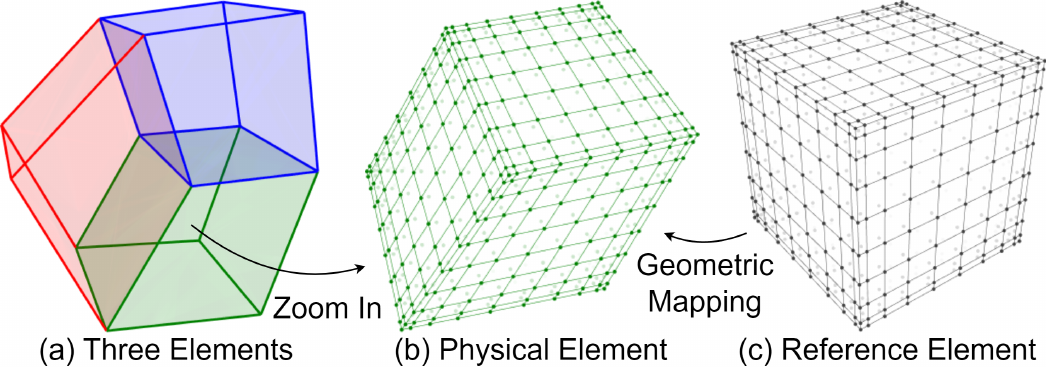
\includegraphics[width=\linewidth]{figs/raster300/d3-three-elements.png}
    \caption{Hybrid organization of high-order element data. (a) Physical elements have irregular global connectivity. (b) Each physical element contains a deformed tensor-product arrangement of data points. (c) Every physical element is obtained by geometrically mapping a common reference element.}
    \label{fig:characterizing-hohs}
\end{figure}

Within each dataset considered in this work, every element contains the same tensor-product arrangement of data points. Their physical coordinates need not be uniformly spaced because the element may be geometrically deformed. Figure~\ref{fig:characterizing-hohs}(b) shows a physical element containing $10\times10\times10$ points. For clarity, only points near its three visible faces are highlighted.

The local indexing shared by all elements originates from a reference element with a canonical shape. Within the reference element, point coordinates along each dimension are selected from a fixed set. Gauss--Lobatto--Legendre (GLL) points are a common choice in high-order element methods~\cite{fischer2022nekrs,marin2016spectral}. They include the element boundaries and are nonuniformly spaced, as shown in Figure~\ref{fig:characterizing-hohs}(c). The arrow between Figures~\ref{fig:characterizing-hohs}(c) and~\ref{fig:characterizing-hohs}(b) represents the geometric mapping from the reference element to a physical element. Consequently, the same local index identifies the same reference-space position across elements even when the corresponding physical coordinates differ.

\subsection{Problem Formulation}\label{sec:problem formulation:metrics}

\begin{figure}[htb]
    \centering
    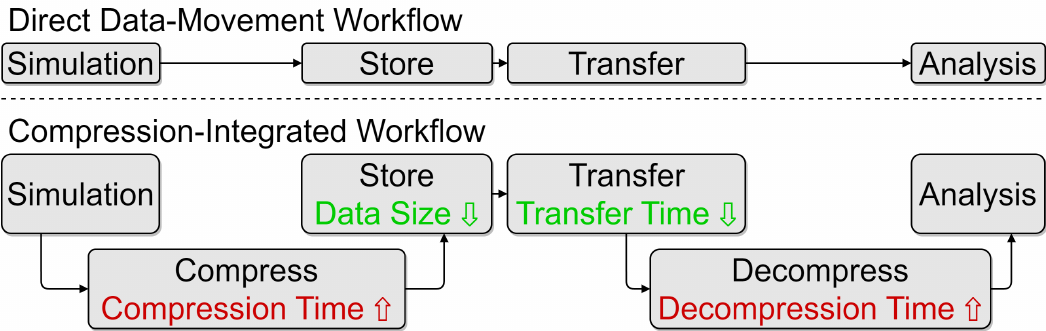
\includegraphics[width=\linewidth]{figs/raster300/d3-end-to-end.png}
    \caption{Comparison of direct and compression-integrated data-movement workflows. Compression reduces storage and transfer costs while introducing compression and decompression overhead.}
    \label{fig:end-to-end}
\end{figure}

Given a field $X$ and an absolute error bound $\varepsilon_{\mathrm{abs}}$, a compressor produces a bitstream $B$, from which the decompressor reconstructs a field $\widehat{X}$. We require a strict pointwise error guarantee:
\begin{equation}
\max_{e,i,j,k}|x_{e,i,j,k}-\widehat{x}_{e,i,j,k}|\leq\varepsilon_{\mathrm{abs}}.
\end{equation}
The corresponding value-range-based relative error bound is $\varepsilon_{\mathrm{rel}}=\varepsilon_{\mathrm{abs}}/R$, where $R=\max(X)-\min(X)$. Different physical fields may have different ranges, accuracy requirements, and downstream uses. We therefore compress each field independently and allow its error bound to be selected separately.

The pointwise error bound controls the largest reconstruction error but does not determine the overall distortion. We therefore quantify overall data quality using peak signal-to-noise ratio (PSNR), defined as $20\log_{10}(R/\mathrm{RMSE})$. We define normalized RMSE (NRMSE) and normalized MAE (NMAE) as $\mathrm{RMSE}/R$ and $\mathrm{MAE}/R$, respectively.

To characterize symbol compressibility, we also report the empirical zero-order entropy of the quantized symbols. For a scalar quantity $z$ quantized under an absolute error bound $\varepsilon$, we define the quantized symbol $q=\operatorname{round}(z/(2\varepsilon))$ and $H=-\sum_qp_q\log_2p_q$, where $p_q$ is the observed frequency of symbol $q$. For prediction analysis, $z=x-\widetilde{x}$ is the prediction error. Entropy is reported in bits per symbol. It is not the final bit rate and excludes metadata and dependencies among symbols.

At a given PSNR, our first objective is to minimize the size of $B$. We report storage reduction using either compression ratio (CR), defined as the original data size divided by the compressed size, or bit rate (BR), defined as the average number of compressed bits per data value.

Our second objective is to reduce end-to-end data-movement time under a prescribed pointwise error bound. As illustrated in Figure~\ref{fig:end-to-end}, this requires balancing compression and decompression overhead against the transfer savings from a smaller bitstream. To capture this tradeoff beyond codec throughput, we also measure end-to-end runtime.
